%--------------------------------------------------------------------------------------------------
%
\chapter{Experiments}\label{chap:experiments}
%--------------------------------------------------------------------------------------------------

\section{Experiments}\label{chap:experiments:horst}
In practice, we observe a linear convergence (Figures~\ref{fig:qcqpConvVar}
and \ref{fig:qcqpConvFix}). In Figure~\ref{fig:qcqpConvVar}, we
generated $1000$ random\footnote{We used the random Gram matrix method
to generate random problem instances; for details see
Section~\ref{subsec:syndata}} instances of matrices $A$ with block
structure $b = \left(2,2,2,2,2\right)$. For each matrix, we generated
a starting point $x_0$ and ran the algorithm. The plot depicts the
solution change rate on a logarithmic scale ($log_{10}
\frac{\norm{x_{old} - x}}{\norm{x}}$). We observe linear convergence
over a wide range of rates of convergence (slopes of the
lines). Figure~\ref{fig:qcqpConvFix} shows the convergence properties
for a fixed matrix $A$ with several random initial vectors $x_0$. The
problem exhibits a global
and a local solution. For $65\%$ of the initial vectors, the global solution was reached (versus $35\%$ for the local solution). Note that the global
solution paths tend to converge faster (the average global solution path slope is  $-0.08$, compared  to $-0.05$ for the local solution paths).

%\begin{figure*}[htbp]
%  \centering
%\subfigure[Convergence plot ($1000$ random matrices $A$, one random $x_0$ per problem instance)]{\label{fig:qcqpConvVar}
%    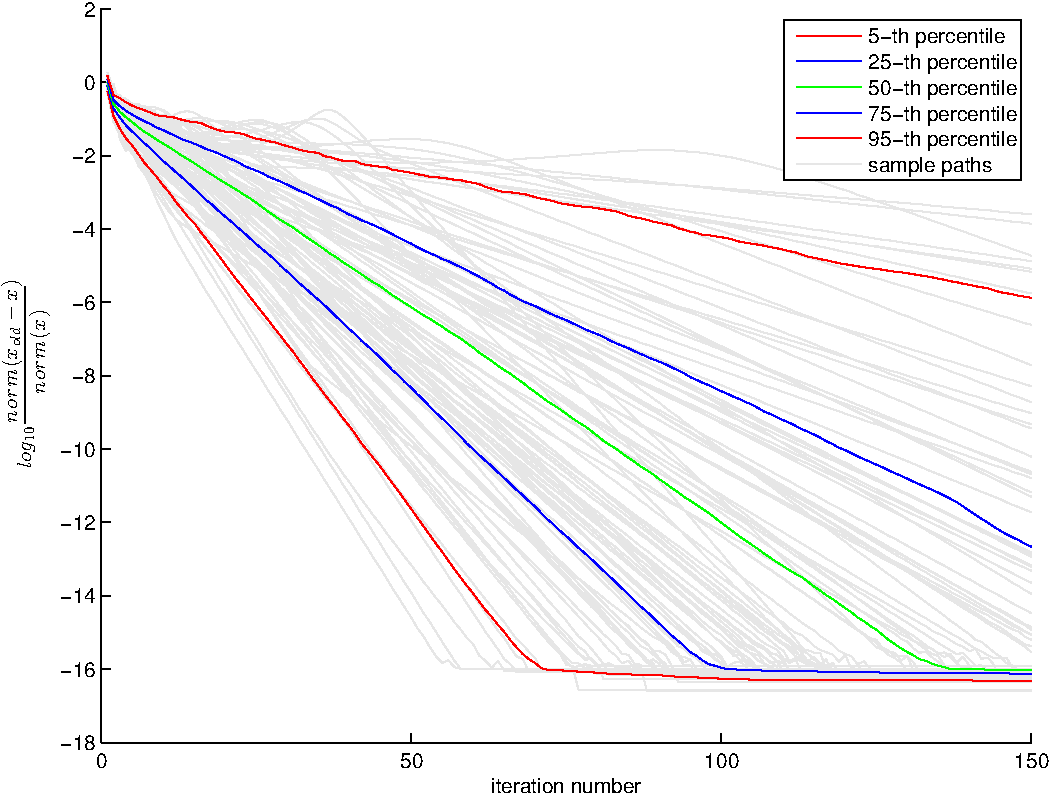
\includegraphics[width=0.47\textwidth]{convergenceBoxPlotDifferentA.pdf}
%}
%\subfigure[Convergence plot (single random $A$, $1000$ random initial vectors $x_0$)]{\label{fig:qcqpConvFix}
%    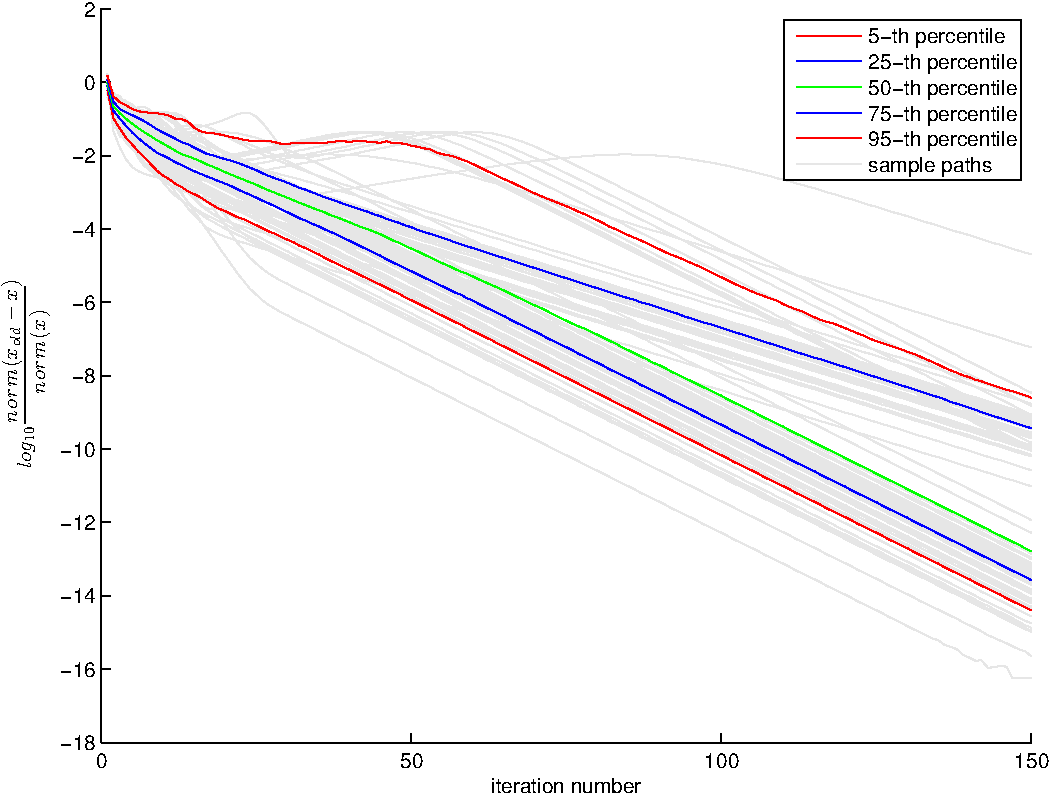
\includegraphics[width=0.47\textwidth]{convergenceBoxPlotFixedA.pdf}
%}
%\end{figure*}


\section{Experiments}\label{sec:experiments}

We evaluated the local and global approaches on two scenarios: a performance
analysis on synthetic data and the performance on finding a common
representation of a cross-lingual collection of documents.
%, performance of the methods on the task of signal blind source separation and an exploratory analysis of sensor network data.

\subsection{Synthetic data}\label{subsec:syndata}
We generated several MCCA problem instances by varying the number
of views and number the of dimensions per view in order to
compare the performance of local search methods and the proposed
SDP relaxation. The goal of these experiments was to see
under which conditions and how often do the global bounds
provide useful information.

 Let $m$ denote the number of views
(sets of variables) and $n_i$ denote the dimensionality of $i$-th
view and $N := \sum_i n_i$. In all cases, we used the same number
of dimensions per view ($n_1 = n_2 = \cdots = n_m$). We used
three different methods to generate random correlation matrices.

The first method,  the \textbf{random Gram matrices} method (see
\cite{Holmes:1991:RCM:105724.105730}, \cite{Bendel_Mickey_78}) ,
generates the correlation matrices by sampling $N$ vectors $v_1,
\ldots, v_n$ for an $N$-dimensional multivariate Gaussian
distribution (centered at the origin, with an identity covariance
matrix), normalizing them and computing the correlation matrix $C
= \left[c_{i,j}\right]_{N \times N}$ as $c_{i,j} := v_i' \cdot v_j$.
%
The second method,  the \textbf{random spectrum} method,
samples the eigenvalues $\lambda_1,\ldots,\lambda_N$ uniformly
from a simplex ($\sum_{i=1}^{N} \lambda_i = N$) and generates a
random correlation matrix with the prescribed eigenvalues (see
\cite{Bendel_Mickey_78}).
%
The final method, the \textbf{random 1-dim structures} method,
generates a correlation matrix that has an approximately (due to
noise) single-dimensional correlation structure. We
generate a random $m$ dimensional Gram matrix $B$, and insert
it into an $N\times N$ identity matrix according to the block
structure to obtain a matrix $C_0$. That is, we set $C_0\left(i,j\right) = \delta\left(i,j\right)$,
where $\delta$ is the Kronecker delta. For $I,J = 1\ldots,m$, we
override the entries $$C_0\left(1+ \sum_{i=1}^{I-1}n_i, 1+
\sum_{i=1}^{J-1}n_i\right) = B\left(I,J\right),$$ where we used $1$-based
indexing. We then generate a random Gram matrix $D \in
\RR^{N\times N}$ and compute the final correlation matrix as $C
= \left(1- \epsilon\right)C_0 + \epsilon D$.
 In our experiments, we set
$\epsilon = 0.001$.

The purpose of using a random spectrum method
is that as the dimensionality increases, random vectors tend to
be orthogonal, hence the experiments based on random Gram
matrices might be less informative. As the experiments show, the
local method suffers  when all $n_i = 1$ (an
instance of a BQO problem). By using the approximately
1-dimensional correlation matrix sampling, we investigated how the
problem behaves when $n_i > 1$.
%
In all cases, we perform a final step that involves computing the
per-view Cholesky decompositions of variances and change of basis
%as we showed when we arrived to QCQP reformulation in equation
(as in \ref{eq:qcqp}).


The experiments are based on varying the number of sets of
variables, $m$ and the dimensionality $n_i$. For each sampling
scenario and each choice of $m$ and $n_i$, we generated $100$
experiments, and computed $1000$ solutions based on Algorithm
\ref{algorithm:horst},  the SDP solution (and respective
global bounds), and examined the frequencies of the following
events:
\begin{itemize}
\item a \textbf{duality gap} candidate detected (Tables
\ref{tb:rg}, \ref{tb:rs}, \ref{tb:r1d} (a))
\item \textbf{local convergence} detected (Tables \ref{tb:rg}, \ref{tb:rs},
\ref{tb:r1d} (b))
\item when a local solution is worse
than the SDP-based \textbf{lower bound} (Tables \ref{tb:rg},
\ref{tb:rs}, \ref{tb:r1d} (c)).
\end{itemize}
The possibility of a duality gap is
detected when the best local solution is lower than $1\%$ of the
SDP bound. In this case, the event indicates only the possibility
of duality gap -- it might be the case that further local
algorithm restarts would close the gap. Local convergence
is detected when the objective value of two local solutions
differs relatively by at least $10\%$ and absolutely at least by
$0.1$ (both criteria must be satisfied
simultaneously). Finally, the event of a local solution being
below the SDP lower bound means that it is below
$\frac{2}{\pi}$ of the optimal objective value of the SDP
relaxation.

We find that regardless of the generation technique, the lower
SDP bound is useful only when $n_i = 1$ (Table \ref{tb:rg},
\ref{tb:rs}, \ref{tb:r1d} (c)) and the results are similar for
different choices of $m$. There are, however rare instances (less
than $0.1\%$) where the lower bound is useful for $n_i = 2$ and
even rarer (less than $0.01\%$) for $n_i = 3$.

The chance of local convergence increases as the number of views
$m$ increases which can be consistently observed for all choices
of $n_i$ and sampling strategies. Generating a generic  problem where the
local algorithm  converges to a local solution is less
likely as the dimensionality increases
(Tables \ref{tb:rg}, \ref{tb:rs}).
%
%
%\textcolor{red}{Nasledni odstavek ne razumem}
%\textcolor{red}{Sem popravil. A je OK? Jan}
In the case of noisy embeddings of a 1-dimensional correlation structures, the dependence on $n_i$
behaves differently: the local convergence (see Table \ref{tb:r1d_lc}) for the case $\left(m=5, n_i=3\right)$ is more likely than for the case $\left(m=5, n_i =2\right)$. This is unexpected as in the general case, increasing $n_i$ reduces that chance of local convergence, see Table \ref{tb:rs_lc}, Table \ref{tb:rg_lc}.

The relationship between $m$ and $n_i$ and the possibility of a
duality gap behaves similarly as local convergence -
increasing $m$ increases it and increasing $n_i$ decreases it (Table \ref{tb:rg_dg}, Table \ref{tb:rs_dg}),
except in the case of noisy 1-dim correlation structures, where
we observe the same anomaly when $n_i = 2$ (Table \ref{tb:r1d_dg}).

Therefore we have demonstrated that there exist sets of problems with nonzero
measure where the SDP bounds give useful information.
%
%\begin{table}
%\begin{center}
%\caption{\label{tb:rg} Random Gram matrix sampling}
%\subtable[Possible duality gap]{\label{tb:rg_dg}
%\centering\begin{tabular}{|l|c|c|c|}
\hline
&\textbf{$n_i$ = 3}&\textbf{$n_i$ = 2}&\textbf{$n_i$ = 1}\\\hline
\textbf{$m$ = 5}&0\%&5\%&17\%\\\hline
\textbf{$m$ = 3}&0\%&0\%&9\%\\\hline
\end{tabular}

%}
%\subtable[Local convergence]{\label{tb:rg_lc}
%\centering\begin{tabular}{|l|c|c|c|}
\hline
&\textbf{$n_i$ = 3}&\textbf{$n_i$ = 2}&\textbf{$n_i$ = 1}\\\hline
\textbf{$m$ = 5}&1\%&5\%&48\%\\\hline
\textbf{$m$ = 3}&0\%&1\%&26\%\\\hline
\end{tabular}

%}
%\subtable[Local solution below lower SDP bound]{\label{tb:rg_lb}
%\centering\begin{tabular}{|l|c|c|c|}
\hline
&\textbf{$n_i$ = 3}&\textbf{$n_i$ = 2}&\textbf{$n_i$ = 1}\\\hline
\textbf{$m$ = 5}&0\%&0\%&14\%\\\hline
\textbf{$m$ = 3}&0\%&0\%&12\%\\\hline
\end{tabular}

%}%
%\end{center}
%\end{table}
%%
%\begin{table}
%\begin{center}
%\caption{\label{tb:rs}Random spectrum sampling}
%\subtable[Possible duality gap]{\label{tb:rs_dg}
%\centering\begin{tabular}{|l|c|c|c|}
\hline
&\textbf{$n_i$ = 3}&\textbf{$n_i$ = 2}&\textbf{$n_i$ = 1}\\\hline
\textbf{$m$ = 5}&0\%&5\%&36\%\\\hline
\textbf{$m$ = 3}&0\%&1\%&20\%\\\hline
\end{tabular}

%}
%\subtable[Local convergence]{\label{tb:rs_lc}
%\centering\begin{tabular}{|l|c|c|c|}
\hline
&\textbf{$n_i$ = 3}&\textbf{$n_i$ = 2}&\textbf{$n_i$ = 1}\\\hline
\textbf{$m$ = 5}&1\%&3\%&50\%\\\hline
\textbf{$m$ = 3}&0\%&0\%&31\%\\\hline
\end{tabular}

%}
%\subtable[Local solution below lower SDP bound]{\label{tb:rs_lb}
%\centering\begin{tabular}{|l|c|c|c|}
\hline
&\textbf{$n_i$ = 3}&\textbf{$n_i$ = 2}&\textbf{$n_i$ = 1}\\\hline
\textbf{$m$ = 5}&0\%&0\%&15\%\\\hline
\textbf{$m$ = 3}&0\%&0\%&16\%\\\hline
\end{tabular}

%}%
%\end{center}
%\end{table}
%%
%\begin{table}
%\begin{center}
%\caption{\label{tb:r1d}Random 1-dim structure sampling}
%\subtable[Possible duality gap]{\label{tb:r1d_dg}
%\centering\begin{tabular}{|l|c|c|c|}
\hline
&\textbf{$n_i$ = 3}&\textbf{$n_i$ = 2}&\textbf{$n_i$ = 1}\\\hline
\textbf{$m$ = 5}&24\%&16\%&23\%\\\hline
\textbf{$m$ = 3}&7\%&4\%&7\%\\\hline
\end{tabular}

%}
%\subtable[Local convergence]{\label{tb:r1d_lc}
%\centering\begin{tabular}{|l|c|c|c|}
\hline
&\textbf{$n_i$ = 3}&\textbf{$n_i$ = 2}&\textbf{$n_i$ = 1}\\\hline
\textbf{$m$ = 5}&9\%&6\%&51\%\\\hline
\textbf{$m$ = 3}&0\%&0\%&31\%\\\hline
\end{tabular}

%}
%\subtable[Local solution below lower SDP bound]{\label{tb:r1d_lb}
%\centering\begin{tabular}{|l|c|c|c|}
\hline
&\textbf{$n_i$ = 3}&\textbf{$n_i$ = 2}&\textbf{$n_i$ = 1}\\\hline
\textbf{$m$ = 5}&0\%&0\%&13\%\\\hline
\textbf{$m$ = 3}&0\%&0\%&15\%\\\hline
\end{tabular}

%}%
%\end{center}
%\end{table}


\subsection{Multilingual document collection}\label{subsec:documents}
%\textbf{Motivation}

Applications of canonical correlation analysis on collections of
documents include: dimensionality reduction, cross-lingual document retrieval and classification
\cite{ccatext} \cite{ccatextdva}, multilingual topic extraction
 \cite{mcca} and news bias detection \cite{ccanewsbias}. In this section, we explore the behavior of
Algorithm \ref{algorithm:horst} with respect to the global
bounds on real data. We start by describing the data and then describe a method to
reduce the dimensionality of the data in order to apply the SDP
bounds.


\noindent\textbf{Dataset and preprocessing}
The experiments were conducted on a subset of EuroParl, Release v3,
\cite{europarl}, a multilingual parallel corpus, where our subset
includes Danish, German, English, Spanish, Italian, Dutch,
Portuguese and Swedish. We first removed all documents
which had one translation or more missing. Documents (each
document is a day of sessions of the parliament) were then
arranged alphabetically and split into smaller documents, such that
each speaker instance represented a separate document.
Therefore, we ended up with $12,000$ documents per
language. These roughly correspond to all speeches between 2.25.1999
and 3.25.1999. We then computed the bag of words (vector space)
\cite{Salton88term-weightingapproaches} model for each language,
keeping unigrams, bigrams and trigrams that occurred
more than thirty times.
%For example: "Mr", "President" and
%"Mr\_President" all occurred more than thirty times in the
%English part of the corpus and they each represent a dimension in
%the vector space.
This resulted in feature spaces with
dimensionality ranging from $50,000$ (English) to $150,000$
(German). Finally, we computed the tf-idf weighting and normalized
every document for each language. Therefore, we obtained
corpus matrices $X^{(i)}$ for each language, where each
matrix has $12,000$ columns and the columns are aligned
($X^{(i)}\left(:,\ell\right)$ and $X^{(j)}\left(:,\ell\right)$ are a translation of
each other). %In section \ref{sec:sumcorextensions} we showed how to
%derive the QCQP problem, given a set of input matrices $X^{(i)}$.

\noindent\textbf{Random projections and multivariate regression}
%experiments: languagesSDP_main
Applying the global (SDP) techniques to these covariance matrices
presents a scalability problem,  both from the large number
of features (words in vocabulary) and the large number of documents. Typical SDP solvers can find solutions to relaxed forms of
QCQPs with up to a few thousand original variables, which is
insufficient in this case, since the primal representation results in hundreds of thousands of dimensions, and the dual representation results in $25,000$ dimensions (five languages, each containing $5000$ training documents).


 To address this issue,  we
reduce the dimensionality of the feature vectors, resulting in
tractable SDP problem dimensions.
%
One way to analyze a monolingual document collection is to
perform a singular value decomposition of the corpus matrix, a
technique referred to as Latent Semantic Indexing
(LSI)\cite{lsi}. A set of largest singular vectors can be used as
a new document basis for dimensionality reduction. Expressing the
documents with the basis of $k$ largest singular vectors is
optimal with respect to Frobenious norm reconstruction error. If
computing the basis is too expensive, one can generate a random
larger set of basis vectors that achieve similar reconstruction
errors. However, this random projection basis is not
informative in the same sense as the LSI basis is (topics extracted by LSI reflect which topics are
relevant for the corpus, as opposed to random topics).

A variant of LSI for multiple languages, Cross-Lingual LSI
(CL-LSI)\cite{cl_lsi}, first joins all feature spaces thus
obtaining a single multilingual corpus matrix (single language
corpus matrices are stacked together). CL-LSI then proceeds as
standard LSI by computing the singular value decomposition (SVD) of the
multilingual corpus matrix.
%
We experimentally observed that the number
of random projections needed to approximate the decomposition in CL-LSI and thus capture
multi-lingual topics is prohibitively large - while a relatively small number
of random projections is needed to capture the variance in each language, a large
number of random projections is needed to approximate all the cross-covariance matrices simultaneously.
Generating random subspaces with a fixed $k$ sequentially over each language becomes harder with each language.
The probability of generating a subspace for the $m$-th language that is well correlated to the preceding languages decreases
as $m$ increases.

Our approach is based on the following idea. Generate a set of random vectors for one language and use Canonical Correlation Analysis Regression (CCAR)\cite{ccar} (a method similar to ridge regression) to find their representatives in the other languages. Repeat the procedure for each of the remaining languages to prevent bias to a single language. We hypothesize that restricting our search in the spaces spanned by the constructed bases still leads to good solutions. The procedure is detailed in Algorithm \ref{algorithm:rpgen}.

Let $m$ be the number of vector spaces corresponding to different
languages and $n_i$ the dimensionality of the $i-th$ vector
space. Let $X^{(i)} \in \RR^{n_i \times N}$ represent the aligned
document matrix for the $i$-th language.



\begin{algorithm}
\caption{Random projections basis generation}
\label{algorithm:rpgen}
{\bf Input:} $X^{(1)},\ldots X^{(m)}$, $\gamma$ - the regularization coefficient, $k$ - \# of projections/block
\begin{algorithmic}
\FOR{$i = 1$ to $m$}
\STATE $P_{(i,i)} :=$ random $n_i \times k$ matrix with elements sampled $i.i.d.$ from standard normal distribution.
\STATE Re-scale each column of $P_{(i,i)}$ so that its norm is equal to $\sqrt{\frac{n_i}{k}}$.
\FOR{$j = 1$ to $m$}
\IF {$j = i$}
 \STATE continue
\ENDIF
\STATE  $\alpha_{(i,j)} :=  \left(\left(1-\gamma\right) X^{(j)} X^{(j)T} + \gamma  I_j \right)^{-1}$
\STATE  $P_{(i,j)} :=  \alpha_{(i,j)} X^{(j)} X^{(i)T}  P_{(i,i)},$ where $I_j$ is the $n_j \times n_j$ identity matrix.
%\STATE  $P_{(i,j)} :=   \left(\left(1-\gamma\right) X^{(j)} X^{(j)T} + \gamma  I_j \right)^{-1} X^{(j)} X^{(i)T}  P_{(i,i)},$ where $I_j$ is the $n_j \times n_j$ identity matrix.
\ENDFOR
\ENDFOR
\\
\end{algorithmic}
{\bf Output:} matrices $P_{(i,j)} \;\text{for}\; i,j = 1,\ldots,m$
\end{algorithm}

The matrices $P_{(i,1)}, \ldots, P_{(i,m)}$ form the bases of
vector spaces corresponding to $X^{(1)},\ldots, X^{(m)}$. Let
$P_i := \left[P_{(1,i)}, \ldots, P_{(m,i)}\right]$ denote the full basis for
the $i$-th language.
We now experimentally address two questions: does the restricted
space enable us to find \emph{stable patterns} and how informative the SDP
bounds are. Stable patterns are represented by highly correlated directions
in both the training and in independent test sets.

%languagesSDP
%languagesSDP_main
%languageSDP339256474618

%languagesSDP_main(5000, 5, 50, 1000);
%      regprimalS: [0.0100 0.1000 0.5000 0.9000 0.9900]
%     ranprojregS: [0.1000 0.5000 0.9000 0.9900]
%            nexp: 10
%    ntrainPrimal: 5000
%      ntrainDual: 30
%           nview: 5
%        nranproj: 50
%        testsize: 1000
%      resultName: 'languageSDP339256474618'


\noindent\textbf{Experiments}
 The experiments were conducted on the set of five EuroParl
 languages: English, Spanish, German, Italian and Dutch. We set
 $k = 10$ which corresponds to $n_i = 50$ dimensions per view, so
 the QCQP matrix will be of size $250 \times 250$. We randomly
 select $5000$ training documents and $1000$ test documents.  For
 a range of random projection regularization parameters $\gamma$,
 we compute the mappings $P_i$ (based on the train set) and
 reduce the dimensionality of the train and test sets. Then, for
 a range of QCQP regularization parameters $\kappa$, we set up the
 QCQP problem, compute $1000$ local solutions (by Horst
 algorithm) and solve the SDP relaxation. The whole procedure is
 repeated $10$ times.

For each $(\gamma, \kappa)$ pair, we measured the sum of
correlations on the test and train sets. Table
\ref{tb:textTrainTestSumcor} shows the sums of correlations
averaged over $10$ experimental trials. The maximal possible sum
of correlations for five datasets is $\binom{5}{2} = 10$.
We observe that regularizing the whole optimization problem is
not as vital as regularizing the construction of random
projection vectors. This is to be expected since finding the
random projection vectors involves a regression in a high
dimensional space as opposed to solving a lower dimensional
QCQP. Selecting $\gamma = 0.1$ leads to perfectly correlated
solutions on the training set for all $\kappa$. This turns out to
be over-fitted when we evaluate the sum of correlations on the
test set - perfect correlations on the training set turn out to be spurious patterns, since they are not present in the test set.
%The test set does not reflect them (sum of correlations ranges between $5.8$ and $7.4$).
Note that higher $\kappa$ values improve the
performance on the test set up to a certain level below
$7.5$. As we increase $\gamma$ to $0.5$, we see a reduction in
overfitting and with $\gamma = 0.9$ we observe stable patterns. Therefore, using
appropriate values, we can reduce the dimensionality of the
original QCQP problem  and still find stable
solutions.  The reduced dimensionality now enables us to investigate
the behavior of the SDP relaxation.
%
For the SDP bounds, we observed behavior that was similar to the high-dimensional synthetic (generic) case. That is
we found that the potential duality gap was very small and that the SDP and the Horst algorithm yielded the same
result. For this reason we omit the SDP results from Table \ref{tb:textTrainTestSumcor}.

%\begin{table}[tbp]
%\begin{center}
%\caption{\label{tb:textTrainTestSumcor} Train and test sum of correlation}
%\subtable[Train set sum of correlations]{\label{tb:trainText}
%\centering\begin{tabular}{|l|c|c|c|c|}
\hline
&\textbf{$\gamma =$0.1}&\textbf{$\gamma =$0.5}&\textbf{$\gamma =$0.9}&\textbf{$\gamma =$0.99}\\\hline
\textbf{$\kappa =$0.01}&10.0&9.8&9.8&9.8\\\hline
\textbf{$\kappa =$0.1}&10.0&9.8&9.8&9.8\\\hline
\textbf{$\kappa =$0.5}&10.0&9.8&9.8&9.8\\\hline
\textbf{$\kappa =$0.9}&10.0&9.8&9.8&9.8\\\hline
\textbf{$\kappa =$0.99}&10.0&9.8&9.7&9.8\\\hline
\end{tabular}

%}
%\subtable[Test set sum of correlations]{\label{tb:testText}
%\centering\begin{tabular}{|l|c|c|c|c|}
\hline
&\textbf{$\gamma =$0.1}&\textbf{$\gamma =$0.5}&\textbf{$\gamma =$0.9}&\textbf{$\gamma =$0.99}\\\hline
\textbf{$\kappa =$0.01}&5.8&8.6&9.6&9.8\\\hline
\textbf{$\kappa =$0.1}&6.2&8.6&9.6&9.8\\\hline
\textbf{$\kappa =$0.5}&7.0&8.6&9.6&9.8\\\hline
\textbf{$\kappa =$0.9}&7.4&8.8&9.6&9.8\\\hline
\textbf{$\kappa =$0.99}&7.4&8.8&9.6&9.8\\\hline
\end{tabular}

%}
%\end{center}
%\end{table}


\section{Evaluation}\label{sec:evaluation}

We will describe the main dataset for building cross-lingual models which is based on Wikipedia and then present two sets of experiments. The first set of experiments
establishes that the hub based approach can deal with language pairs where little or no training data is available. The second set of experiments compares the main approaches
that we presented on the task of mate retrieval and the task of event linking. Finally, we examine how different choices of features impact the event linking performance.

\subsection{Wikipedia Comparable Corpus}

To investigate the empirical performance of the low-rank approximations we will test the algorithms on a large-scale, real-world multilingual dataset that we extracted from Wikipedia by using inter-language links for alignment. This  results in a large number of weakly comparable documents in more than $200$ languages. Wikipedia is a large source of multilingual data that is especially important for the languages for which no translation tools, multilingual dictionaries as Eurovoc~\cite{eurovoc}, or strongly aligned multilingual corpora as Europarl~\cite{europarl} are available. Documents in different languages are related with so called 'inter-language' links that can be found on the left of the Wikipedia page. The Wikipedia is constantly growing. There are currently 12 Wikipedias with more than 1 million %$10^6$
 articles, $52$ with more than 100k %$10^5$
 articles, $129$ with more than 10k articles, and $236$ with more than $1,000$ articles.

Each Wikipedia page is embedded in the page tag. First, we check if the title of the page starts with a Wikipedia namespace (which includes categories and discussion pages) and do not process the page if it does. Then, we check if this is a redirection page and we store the redirect link because inter-language links can point to redirection links also. If none of the above applies, we extract the text and parse the Wikipedia markup. Currently, all the markup is removed.

We get inter-language link matrix using previously stored redirection links and inter-language links. If an inter-language link points to the redirection we replace it with the redirection target link. It turns out that we obtain the matrix $M$ that is not symmetric, consequently the underlying graph is not symmetric. That means that existence of the inter-language link in one way (i.e., English to German) does not guarantee that there is an inter-language link in the reverse direction (German to English). To correct this we transform this matrix to be symmetric by computing $M+M^T$ and obtaining an undirected graph. In the rare case that after symmetrization we have multiple links pointing from the document, we pick the first one that we encountered. This matrix enables us to build an alignment across all Wikipedia\footnote{https://www.wikipedia.org/ dumps available in 2013} languages.

\subsection{Experiments With Missing Alignment Data}\label{experiments:hubcca}

 In this subsection, we will investigate the empirical performance of hub CCA approach. We will demonstrate that this approach can be successfully applied even in the case of fully missing alignment information.
 To this purpose, we select a subset of Wikipedia languages containing three major languages, English (4,212k articles)--\emph{en} (hub language), Spanish (9,686k articles)--\emph{es}, Russian (9,662k articles)--\emph{ru}, and five minority (in terms of Wikipedia sizes) languages, Slovenian (136k articles)--\emph{sl}, Piedmontese (59k articles)--\emph{pms}, Waray-Waray (112k articles)--\emph{war} (all with about 2 million native speakers), Creole (54k articles)--\emph{ht} (8 million native speakers), and Hindi (97k articles)--\emph{hi} (180 million native speakers). For preprocessing, we remove the documents that contain less than 20 different words (referred to as stubs\footnote{Such documents are typically of low value as a linguistic resource. Examples include the titles of the columns in the table, remains of the parsing process, or Wikipedia articles with very little or no information contained in one or two sentences.}) and remove words occurring in less than 50 documents as well as the top 100 most frequent words (in each language separately). We represent the documents as normalized TFIDF~\cite{Salton88term-weightingapproaches} weighted vectors. The IDF scores are computed for each language based on its aligned documents with the English Wikipedia. The English language IDF scores are based on all English documents for which aligned Spanish documents exist.

The evaluation is based on splitting the data into training and test sets. %(which are described later).
We select the test set documents as all multilingual documents with at least one nonempty alignment from the list: (\emph{hi}, \emph{ht}), (\emph{hi}, \emph{pms}), (\emph{war}, \emph{ht}), (\emph{war}, \emph{pms}). This guarantees that we cover all the languages. Moreover this test set is suitable for testing the retrieval through the hub as the chosen pairs have empty alignments. The remaining documents are used for training. In Table \ref{table:train_test}, we display the corresponding sizes of training and test documents for each language pair.

On the training set, we perform the two step procedure to obtain the common document representation as a set of mappings $P_i$. A test set for each language pair, $test_{i,j} = \{(x_\ell,y_\ell) | \ell = 1:n(i,j)\} $, consists of comparable document pairs (linked Wikipedia pages), where $n(i,j)$ is the test set size. We evaluate the representation by measuring mate retrieval quality on the test sets: for each $\ell$, we rank the projected documents $P_j(y_1),\ldots, P_j(y_{n(i,j)})$ according to their similarity with $P_i(x_\ell)$ and compute the rank of the mate document $r(\ell) = rank(P_j(y_\ell))$. The final retrieval score (between -100 and 100) is computed as: $\frac{100}{n(i,j)} \cdot \sum_{\ell = 1}^{n(i,j)} \left( \frac{n(i,j) - r(\ell)}{n(i,j) -1} -0.5\right)$. A score that is less than 0 means that the method performs worse than random retrieval and a score of 100 indicates perfect mate retrieval. The mate retrieval results are included in Table \ref{table:retrieval}.

We observe that the method performs well on all pairs of languages, where at least 50,000 training documents are available(\emph{en}, \emph{es}, \emph{ru}, \emph{sl}). We note that taking $k = 500$ or $k = 1,000$ multilingual topics usually results in similar performance, with some notable exceptions: in the case of (\emph{ht}, \emph{war}) the additional topics result in an increase in performance, as opposed to (\emph{ht}, \emph{pms}) where performance drops, which suggests overfitting. The languages where the method performs poorly are \emph{ht} and \emph{war}, which can be explained by the quality of data (see Table \ref{table:rank} and explanation that follows). In case of \emph{pms}, we demonstrate that solid performance can be achieved for language pairs (\emph{pms}, \emph{sl}) and (\emph{pms}, \emph{hi}), where only 2,000 training documents are shared between \emph{pms} and \emph{sl} and no training documents are available between \emph{pms} and \emph{hi}. Also observe that in the case of (\emph{pms}, \emph{ht}) the method still obtains a score of 62, even though training set intersection is zero and \emph{ht} data is corrupted, which we will show in the next paragraph.
{
\renewcommand\tabcolsep{3pt}
\begin{table}[h!]
\centering
\caption{Training -- test sizes (in thousands).
The first row represents the size of the training sets used to construct the mappings in low-dimensional language independent space using \emph{en} as a hub. The diagonal elements represent the number of the unique training documents and test documents in each language.
}
\label{table:train_test}
{
\small
\begin{tabular}{c|c|c|c|c|c|c|c|c|}
&	en&	es&	ru&	sl&	hi&	war&	ht&	pms\\\cline{1-9}
en&	671~-~4.64&	463~-~4.29&	369~-~3.19&	50.3~-~2&	14.4~-~2.76&	8.58~-~2.41&	 17~-~2.32&	16.6~-~2.67\\
\cline{2-9}
es&	\multicolumn{1}{c|}{}	&	463~-~4.29&	187~-~2.94&	28.2~-~1.96&	8.72~-~2.48&	 6.88~-~2.4&	13.2~-~2&	 13.8~-~2.58\\
\cline{3-9}
ru&	\multicolumn{2}{c|}{}	&	369~-~3.19&	29.6~-~1.92&	9.16~-~2.68&	2.92~-~1.1&	 3.23~-~2.2&	10.2~-~1.29\\
\cline{4-9}
sl&	\multicolumn{3}{c|}{}	&	50.3~-~2&	3.83~-~1.65&	1.23~-~0.986&	0.949~-~1.23&	 1.85~-~0.988\\
\cline{5-9}
hi&	\multicolumn{4}{c|}{}	&	14.4~-~2.76&	0.579~-~0.76&	0.0~-~2.08&	0.0~-~0.796\\
\cline{6-9}
war&	\multicolumn{5}{c|}{}	&	8.58~-~2.41&	0.043~-~0.534&	0.0~-~1.97\\
\cline{7-9}
ht&	\multicolumn{6}{c|}{}	&	17~-~2.32&	0.0~-~0.355\\
\cline{8-9}
pms&	\multicolumn{7}{c|}{}	&	16.6~-~2.67\\
\cline{9-9}
\end{tabular}
}
\end{table}
}

{
\renewcommand\tabcolsep{3pt}
\begin{table}[h!]
\caption{Pairwise retrieval, 500 topics on the left -- 1,000 topics on the right}\label{table:retrieval}
\begin{center}
\begin{tabular}{|c|c|c|c|c|c|c|c|c|}
\cline{1-9}
&	en&	es&	ru&	sl&	hi&	war&	ht&	pms\\\cline{1-9}
en&	    &	98~-~98&	95~-~97&	97~-~98&	82~-~84&	76~-~74&	53~-~55&	 96~-~97\\
\cline{1-9}
es&	97~-~98&	&	94~-~96&	97~-~98&	85~-~84&	76~-~77&	56~-~57&	96~-~96\\
\cline{1-9}
ru&	96~-~97&	94~-~95&	&	97~-~97&	81~-~82&	73~-~74&	55~-~56&	96~-~96\\
\cline{1-9}
sl&	96~-~97&	95~-~95&	95~-~95&	&	91~-~91&	68~-~68&	59~-~69&	93~-~93\\
\cline{1-9}
hi&	81~-~82&	82~-~81&	80~-~80&	91~-~91&	&	68~-~67&	50~-~55&	87~-~86\\
\cline{1-9}
war&	68~-~63&	71~-~68&	72~-~71&	68~-~68&	66~-~62&	&	28~-~48&	 24~-~21\\
\cline{1-9}
ht&	52~-~58&	63~-~66&	66~-~62&	61~-~71&	44~-~55&	16~-~50&	&	62~-~49\\
\cline{1-9}
pms&	95~-~96&	96~-~96&	94~-~94&	93~-~93&	85~-~85&	23~-~26&	66~-~54&	 \\
\cline{1-9}
\end{tabular}
\end{center}
\end{table}
}

We further inspect the properties of the training sets by roughly estimating the fraction $\frac{rank(A)}{min\left(rows\left(A\right),~cols\left(A\right)\right)}$ for each English training matrix and its corresponding mate matrix, where $rows(A)$ and $cols(A)$ denote the number of rows and columns respectively. The denominator represents the theoretically highest possible rank the matrix $A$ could have. Ideally, these two fractions should be approximately the same - both aligned spaces should have reasonably similar dimensionality. We display these numbers as pairs in Table \ref{table:rank}.

\begin{table}[h]
\caption{Dimensionality drift. Each column corresponds to a pair of aligned corpus matrices between English and another language. The numbers represent the ratio between the numerical rank and the highest possible rank. For example, the column $en -- ht$ tells us that for the English-Creole pairwise-aligned corpus matrix pair, the English counterpart has full rank, but the Creole counterpart is far having full rank.}
\label{table:rank}
\begin{tabular}{|c|c|c|c|c|c|c|}
\cline{1-7}
en -- es     &   en -- ru     &   en -- sl       &     en -- hi &   en -- war      &      en -- ht &   en -- pms\\
\cline{1-7}
0.81 -- 0.89   &  0.8 -- 0.89  &   0.98 -- 0.96    &    1 -- 1  &  0.74 -- 0.56  &      1 -- 0.22  &   0.89 -- 0.38\\
\cline{1-7}
\end{tabular}
\end{table}

It is clear that in the case of the Creole language only at most $22\%$ documents are unique and suitable for the training. Though we removed the stub documents, many of the remaining documents are nearly the same, as the quality of some smaller Wikipedias is low. This was confirmed for the Creole, Waray-Waray, and Piedmontese languages by manual inspection. The low quality documents correspond to templates about the year, person, town, etc. and contain very few unique words.

There is also a problem with the quality of the test data. For example, if we look at the test pair (\emph{war}, \emph{ht}) only 386/534 Waray-Waray test documents are unique but on the other side almost all Creole test documents (523/534) are unique. This indicates a poor alignment which leads to poor performance.
%}

\subsection{Evaluation Of Cross-Lingual Event Linking}
In order to determine how accurately we can predict cluster equivalence, we performed two experiments in a multilingual setting using English, German and Spanish languages for which we had labelled data to evaluate the linking performance. In the first experiment, we tested how well  the individual approaches for cross-lingual article linking perform when used for linking the clusters about the same event. In the second experiment we tested how accurate the prediction model is when trained on different subsets of learning features. To evaluate the prediction accuracy for a given dataset we used 10-fold cross validation.

We created a manually labelled dataset in order to evaluate cross-lingual event linking using two human annotators. The annotators were provided with an interface listing the articles, their content from and top concepts for a pair of clusters and their task was to determine if the clusters were equivalent or not (i.e., discuss same event). To obtain a pair of clusters $(c_i, c_j)$ to annotate, we first randomly chose a cluster $c_i$, used Algorithm~\ref{cluster_merge_algo1} to compute a set of potentially equivalent clusters $C$ and randomly chose a cluster $c_j \in C$. The dataset provided by the annotators contains 808 examples, of which 402 are equivalent clusters pairs and 406 are not. Clusters in each learning example are either in English, Spanish or German. Although Event Registry imports articles in other languages as well, we restricted our experiments to these three languages. We chose only these three languages since they have very large number of articles and clusters per day which makes the cluster linking problem hard due to large number of possible links.

In Section~\ref{sec:models}, we  described three main algorithms for identifying similar articles in different languages. These algorithms were $k$-means, LSI and hub CCA. As a training set, we used common Wikipedia alignment for all three languages. To test which of these algorithms performed best, we made the following test. For each of the three algorithms, we analyzed all articles in Event Registry and for each article computed the most similar articles in other languages. To test how informative the identified similar articles are for cluster linking we then trained three classifiers as described in Section~\ref{algo:features} -- one for each algorithm. Each classifier was allowed to use as learning features \textbf{only} the cross-lingual article linking features for which values are determined based on the selected algorithm ($k$-means, LSI and hub CCA). The results of the trained models are shown in Table~\ref{table:linkingEvalAlgos}. We also show how the number of topics (the dimensions of the latent space) influences the quality, except in the case of the $k$-means algorithm, where only the performance on 500 topic vectors is reported, due to higher computational cost.

We observe that, for the task of cluster linking, LSI and hub CCA perform comparably and both outperform $k$-means.

% AMMR experiments
We also compared the proposed approaches on the task of Wikipedia mate retrieval (the same task as in Section~\ref{experiments:hubcca}). We computed the Average (over language pairs) Mean Reciprocal Rank (AMRR)~\cite{voorhees1999trec}  performance of the different approaches on the  Wikipedia data by holding out $15,000$ aligned test documents and using $300,000$ aligned documents as the training set. Figure~\ref{pic:AMRR} shows AMRR score as the function of the number of feature vectors. It is clear that hub CCA outperforms LSI approach and $k$-means lags far behind when testing on Wikipedia data. The hub CCA approach with $500$ topic vectors manages to perform comparably to the $LSI$-based approach with $1,000$ topic vectors, which shows that the $CCA$ method can improve both model memory footprint as well as similarity computation time.

% number of topics?
Furthermore, we inspected how the number of topics influences the accuracy of cluster linking. As we can see from Table~\ref{table:linkingEvalAlgos} choosing a number of features larger than $500$ barely affects linking performance, which is in contrast with the fact that additional topics helped to improve AMMR, see Figure~\ref{pic:AMRR}. Such differences may have arisen due to different domains of training and testing (Wikipedia pages versus news articles).

% cluster size?
We also analyzed how cluster size influences the accuracy of cluster linking. We would expect that if the tested pair of clusters has a larger number of articles then the classifier should be able to more accurately predict whether the clusters should be linked or not. The reasoning is that the large clusters would provide more document linking information (more articles mean more links to other similar articles) as well as more accurately aggregated semantic information. In the case of smaller clusters, the errors of the similarity models have greater impact which should decrease the performance of the classifier, too. To validate this hypothesis we have split the learning examples into two datasets -- one containing cluster pairs where the combined number of articles from both clusters is below 20 and one dataset where the combined number is 20 or more. The results of the experiment can be seen in Table~\ref{table:linkingEvalAlgosLargeSmall}. As it can be seen, the results confirm our expectations: for smaller clusters it is indeed harder to correctly predict if the cluster pair should be merged or not.

The hub CCA attains higher precision and classification accuracy on the task of linking small cluster pairs than the other methods, while LSI is slightly better on linking large cluster pairs. The gain in precision of LSI over hub CCA on linking large clusters is much smaller than the gain in precision of hub CCA over LSI on linking small clusters. For that reason we decided to use hub CCA as the similarity computation component in our system.

%AMPR as function of the number of feature vectors
%\begin{figure}
%\centering
%% This file was created by matlab2tikz.
% Minimal pgfplots version: 1.3
%
%The latest updates can be retrieved from
%  http://www.mathworks.com/matlabcentral/fileexchange/22022-matlab2tikz
%where you can also make suggestions and rate matlab2tikz.
%
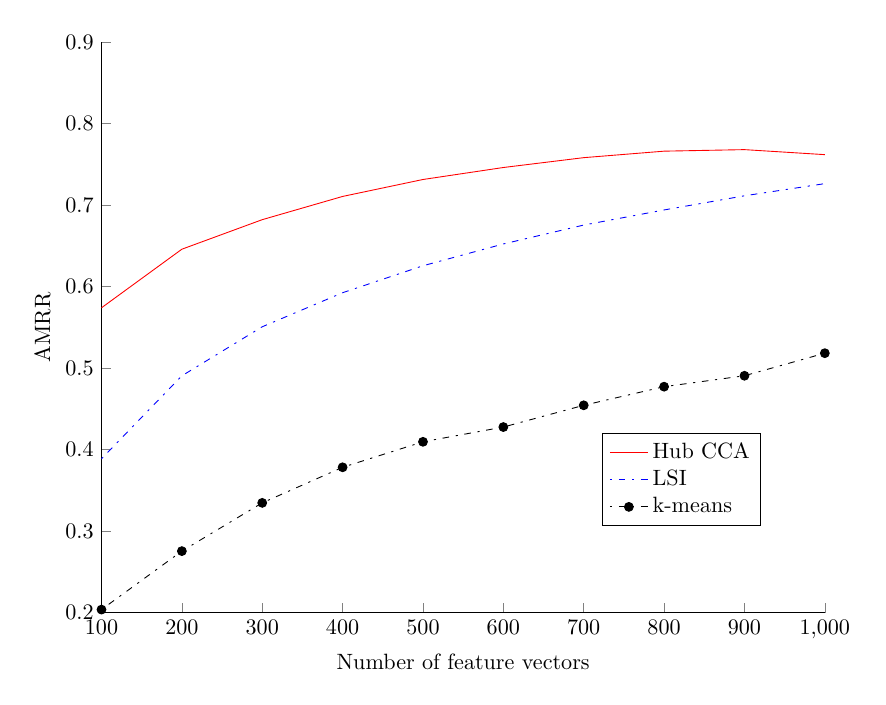
\begin{tikzpicture}[scale=0.8]

\begin{axis}[%
width=4.520833in,
height=3.565625in,
at={(0.758333in,0.48125in)},
scale only axis,
every outer x axis line/.append style={black},
every x tick label/.append style={font=\color{black}},
xmin=100,
xmax=1000,
xlabel={Number of feature vectors},
every outer y axis line/.append style={black},
every y tick label/.append style={font=\color{black}},
ymin=0.2,
ymax=0.9,
ylabel={AMRR},
axis x line*=bottom,
axis y line*=left,
legend style={at={(0.692559,0.152778)},anchor=south west,legend cell align=left,align=left,draw=black}
]
\addplot [color=red,solid]
  table[row sep=crcr]{%
100	0.574094231082746\\
200	0.645978450670063\\
300	0.682226506762222\\
400	0.710722094692085\\
500	0.731517169423203\\
600	0.746223870375363\\
700	0.758312886611436\\
800	0.766279310559898\\
900	0.768159613081689\\
1000	0.76200517888255\\
};
\addlegendentry{Hub CCA};

\addplot [color=blue,dash pattern=on 1pt off 3pt on 3pt off 3pt]
  table[row sep=crcr]{%
100	0.388773162433835\\
200	0.49061571487968\\
300	0.550801867794634\\
400	0.592565604079171\\
500	0.625657099289601\\
600	0.65240747960386\\
700	0.675602522126668\\
800	0.694149727717174\\
900	0.711511053167843\\
1000	0.726455461653153\\
};
\addlegendentry{LSI};

\addplot [color=black,dash pattern=on 1pt off 3pt on 3pt off 3pt,mark=*,mark options={solid}]
  table[row sep=crcr]{%
100	0.203799120889507\\
200	0.275537657758881\\
300	0.334738107118325\\
400	0.378380649062479\\
500	0.409668545430712\\
600	0.427765004442194\\
700	0.454449272479224\\
800	0.477291178317808\\
900	0.490692600634559\\
1000	0.518392823243787\\
};
\addlegendentry{k-means};

\end{axis}
\end{tikzpicture}% 
%\caption{Average of mean reciprocal ranks}
%\label{pic:AMRR}
%\end{figure}

\begin{table}[h]
\caption{Accuracy of cluster linking with 500/800/1,000 topic vectors obtained from different cross-lingual similarity algorithms. The table shows for each of the algorithms the obtained classification accuracy, precision and recall.}
\label{table:linkingEvalAlgos}
\begin{center}
\begin{tabular}{|c|c|c|c|c|}
  \hline
  \cline{1-5}
  Models & Accuracy \% & Precision \% & Recall \% & $F_1$ \% \\ \cline{1-5}
  hub CCA  & 78.2/79.6/80.3 & 76.3/78.0/80.5  & 81.6/82.1/79.9 & 78.9/80.0/80.2
  \\ \cline{1-5}
  LSI      & 78.9/78.7/80.6  & 76.8/77.0/78.7 & 83.3/80.6/83.6 & 79.9/78.8/81.1  \\ \cline{1-5}
 $k$-means & 73.9/-/- & 69.5/-/- & 84.6/-/- &  76.3/-/- \\ \cline{1-5}
 %$k$-means & 73.9/-/-\phantom{/78.7/80.6 } & 69.5/-/-\phantom{/78.7/80.6 }  & 84.6/-/-\phantom{/78.7/80.6 } &  76.3\phantom{/78.7/80.6 }  \\ \cline{1-5}
\end{tabular}
\end{center}
\end{table}

\begin{table}[h]
\caption{Accuracy of cluster linking using $500$ topic vectors on two datasets containing large (left number) and small (right number) clusters. The dataset with small clusters contained the subset of learning examples in which the combined number of articles from both clusters of the cluster pair were below 20. The remaining learning examples were put into the dataset of large clusters.}
\label{table:linkingEvalAlgosLargeSmall}
\begin{center}
\begin{tabular}{|c|c|c|c|c|}
  \hline
  \cline{1-5}
  Models & Accuracy \% & Precision \% & Recall \% & $F_1$ \% \\ \cline{1-5}
  hub CCA  & 81.2 - 77.8 & 80.5 - 74.5 & 91.3 - 57.5 & 85.6 - 64.9 \\ \cline{1-5}
  LSI      & 82.8 - 76.4 & 81.3 - 70.9 & 93.1 - 57.5 & 86.8 - 63.5 \\ \cline{1-5}
 $k$-means & 75.5 - 71.2 & 72.8 - 70.8 & 95.3 - 36.2 & 82.5 - 47.9 \\ \cline{1-5}
\end{tabular}
\end{center}
\end{table}

In the second experiment, we evaluate how relevant individual groups of features are to correctly determine cluster equivalence. For this purpose, we computed accuracy using individual groups of features, as well as using different combination of groups. Since hub CCA had the best  performance of the three algorithms, we used it to compute the values of the cross-lingual article linking features. The results of the evaluation are shown in Table~\ref{table:linkingEval}. We can see that using a single group of features, the highest prediction accuracy can be achieved using  concept-related features. The classification accuracy in this case is 88.5\%. By additionally including also the cross-lingual article linking features, the classification accuracy rises slightly to 89.4\%. Using all three groups of features, the achieved accuracy is 89.2\%.

To test if the accuracy of the predictions is language dependent we have also performed the evaluations separately on individual language pairs. For this experiment we have split the annotated learning examples into three datasets, where each dataset contained only examples for one language pair. When training the classifier all three groups of features were available. The results are shown in Table~\ref{table:langPairEval}. We can see that the performance of cluster linking on the English-German dataset is the highest in terms of accuracy, precision, recall and $F_1$. The performance on the English-Spanish dataset is comparable to the performance on the English-German dataset, where the former achieves higher recall (and slightly higher $F_1$ score), while the latter achieves higher precision. A possible explanation of these results is that the higher quantity and quality of English-German language resources leads to a more accurate cross-lingual article similarity measure as well as to a more extensive semantic annotation of the articles.

Based on the performed experiments, we can make the following conclusions. The cross-lingual similarity algorithms provide valuable information that can be used to identify clusters that describe the same event in different languages. For the task of cluster linking, the cross-lingual article linking features are however significantly less informative compared to the concept-related features that are extracted from the semantic annotations. Nevertheless, the cross-lingual article similarity features are very important for two reasons. The first  is that they allow us to identify for a given cluster a limited set of candidate clusters that are potentially equivalent. This is a very important feature since it reduces the search space by several orders of magnitude. The second reason these features are important is that concept annotations are not available for all articles as the annotation of news articles is computationally intensive and can only be done for a subset of collected articles. The prediction accuracies for individual language pairs are comparable although it seems that the achievable accuracy correlates with the amount of available language resources.


\begin{table}[h]
\caption{The accuracy of the classifier for story linking using different sets of learning features.}
\label{table:linkingEval}
\begin{center}
\begin{tabular}{|c|c|c|c|c|}
  \hline
  \cline{1-5}
  Features & Accuracy \% & Precision \% & Recall \% & $F_1$ \%  \\ \cline{1-5}
  hub CCA            & $78.3 \pm 5.9$ & $78.2 \pm  7.0$ & $78.9 \pm  5.2$ & $78.4 \pm  5.5$ \\ \cline{1-5}
  Concepts           & $88.5 \pm 2.7$ & $88.6 \pm  4.8$ & $88.6 \pm  2.2$ & $88.5 \pm  2.4$ \\ \cline{1-5}
  Misc               & $54.8 \pm 6.7$ & $61.8 \pm 16.5$ & $58.2 \pm 30.2$ & $52.4 \pm 13.0$ \\ \cline{1-5}
  hub CCA + Concepts & $89.4 \pm 2.5$ & $89.4 \pm  4.6$ & $89.6 \pm  2.4$ & $89.4 \pm  2.3$ \\ \cline{1-5}
  hub CCA + Misc     & $78.8 \pm 5.0$ & $78.9 \pm  7.1$ & $79.4 \pm  4.6$ & $79.0 \pm  4.5$ \\ \cline{1-5}
  Concepts + Misc    & $88.7 \pm 2.6$ & $88.8 \pm  4.6$ & $88.8 \pm  2.2$ & $88.7 \pm  2.3$ \\ \cline{1-5}
  All                & $89.2 \pm 2.6$ & $88.8 \pm  4.9$ & $90.1 \pm  1.9$ & $89.3 \pm  2.3$ \\ \cline{1-5}
  \hline
\end{tabular}
\end{center}
\end{table}

\begin{table}[h]
\caption{The accuracy of the classifier for story linking on training data for each language pair separately using all learning features.}
\label{table:langPairEval}
\begin{center}
\begin{tabular}{|c|c|c|c|c|}
  \hline
  \cline{1-5}
  Language pair & Accuracy \% & Precision \% & Recall \% & $F_1$ \% \\ \cline{1-5}
  en, de & $91.8 \pm 5.5$ & $91.7 \pm  6.3$ & $93.7 \pm  6.3$ & $92.5 \pm  5.1$ \\ \cline{1-5}
  en, es & $87.7 \pm 5.4$ & $87.7 \pm  7.4$ & $88.5 \pm  9.8$ & $87.6 \pm  5.9$ \\ \cline{1-5}
  es, de & $88.6 \pm 4.3$ & $89.7 \pm  9.1$ & $84.3 \pm 11.9$ & $85.9 \pm  6.0$ \\ \cline{1-5}
  \hline
\end{tabular}
\end{center}
\end{table}

\subsection{Remarks on the scalability of the implementation}

One of the main advantages of our approach is that it is highly scalable. It is fast, very robust to quality of training data, easily extendable, simple to implement and has relatively small hardware requirements. The similarity pipeline is the most computationally intensive part and currently runs on a machine with two Intel Xeon E5-2667 v2, 3.30GHz processors with 256GB of RAM. This is sufficient to do similarity computation over a large number of languages if needed. It currently uses Wikipedia as a freely available knowledge base and experiments show that the similarity pipeline dramatically reduces the search space when linking clusters.

Currently, we compute similarities over $24$ languages with tags: \emph{eng}, \emph{spa}, \emph{deu}, \emph{zho}, \emph{ita}, \emph{fra}, \emph{rus}, \emph{swe}, \emph{nld}, \emph{tur}, \emph{jpn}, \emph{por}, \emph{ara}, \emph{fin}, \emph{ron}, \emph{kor}, \emph{hrv}, \emph{tam}, \emph{hun}, \emph{slv}, \emph{pol}, \emph{srp}, \emph{cat}, \emph{ukr} but we support any language from the top $100$ Wikipedia languages. Our data stream is Newsfeed (http://newsfeed.ijs.si/) which provides 430k unique articles per day. Our system currently computes 2 million similarities per second, that means that we compute $16 \cdot 10^{10}$ similarities per day. We
store one day buffer for each language which requires 1.5 GB of memory with documents   stored as 500-dimensional vectors. We  note that the time complexity of the similarity computations scales linearly with dimension of the feature space and does not  depend on number of languages. For each article, we compute the top $10$  most similar ones in every other language.

For all linear algebra matrix and vector operations, we use high performance numerical linear algebra libraries as BLAS, OPENBLAS and Intel MKL, which currently allows us to process more than one million articles per day.
In our current implementation, we use the variation of the hub approach. Our projector matrices are of size $500\times 300,000,$ so every projector takes about $1.1$ GB of RAM. Moreover, we need proxy matrices of size $500\times500$ for every language pair. That is 0.5 GB for $24$ languages and $9.2$ GB for $100$ languages. All together we need around 135 GB of RAM for the system with 100 languages.
 Usage of proxy matrices enables the projection of all input documents in the common space and handling language pairs with missing or low alignment. That enables us to do block-wise similarity computations further improving system efficiency. Our code can therefore be easily parallelized using matrix multiplication rather than performing more matrix - vector multiplications. This speeds up our code by a factor of around $4.$ In this way, we obtain some caching gains and ability to use vectorization.
Our system is also easily extendable. Adding a new language requires the  computation of  a projector matrix and proxy matrices with all other already available languages.


